%%%% Better Poster latex template example v1.0 (2019/04/04)
%%%% GNU General Public License v3.0
%%%% Rafael Bailo
%%%% https://github.com/rafaelbailo/betterposter-latex-template
%%%% 
%%%% Original design from Mike Morrison
%%%% https://twitter.com/mikemorrison

\documentclass[a1paper]{betterposter}

\setlength{\leftbarwidth}{0.22\paperwidth}

\usepackage{siunitx}
\sisetup{detect-all}
\usepackage{textcomp}

\usepackage{tikz}
\usetikzlibrary{matrix, positioning, calc, shapes, intersections, through, quotes, angles}

\usepackage{pgfplots}
\usepgfplotslibrary{groupplots}
\pgfplotsset{compat=newest, scale only axis, width = 5cm, height = 5cm, every axis plot/.append style={smooth, thick, no markers}}

\usepackage{tikzscale}

\begin{document}	
\betterposter{

    \maincolumn{

        Calculating \textbf{sensitivity} in\\
        imperfect eyes may be \textbf{inaccurate}.\\
        \\
        \textbf{Ray tracing} sensitivity is superior\\
        to the \textbf{standard model}.
    }{

        \qrcode{img/qrcode}{img/smartphoneWhite}{
            \textbf{Scan or take a picture} for 
            \\the original paper, ray tracer, and this poster
        }
    }

}{

    \title{Sensitivity in\\imperfect eyes}

    \author{Yakir Luc Gagnon\textsuperscript{1}, Daniel Speiser\textsuperscript{2}, and Dan-Eric Nilsson\textsuperscript{1}}

    \institution{\textsuperscript{1} Lund Vision Group, Department of Biology, Lund University, Sweden}
    \institution{\textsuperscript{2} Speiser Lab, College of Arts and Sciences, Univesity of South Carolina, SC, USA}

    \textbf{Visual sensitivity depends on:}
    \begin{enumerate}
        \item How much light reaches the central photoreceptor,
        \item and how much of that light gets absorbed by that receptor. 
    \end{enumerate}

    \textbf{The standard model for sensitivity assumes that:}
    \begin{itemize}
        \item All light that passes the aperture terminates at the central photoreceptor.
        \item On- and off-axis targets focus the same way.
        \item Light passes straight through the full length of the receptor.
    \end{itemize}

    \textbf{But aberrated eyes break those assumptions:}
    \begin{itemize}
        \item Imperfect optics defocus the light.
        \item Coma: changing the viewing angle changes the focus.
        \item Off-axis light does not pass through the whole receptor.
    \end{itemize}

    We used the eyes of scallops as an example of an aberrated visual system. The ray traced sensitivity of their eyes was much lower than the standard model one. 

    \vfill

    \begin{center}
        \includegraphics[width=0.75\textwidth]{img/comparesmall}
    \end{center}

    \vfill

    \begin{center}
        
\includegraphics[height = 2.5cm]{img/lundlogo}
        
\includegraphics[height = 2.5cm]{img/europeancommission}
        
\includegraphics[height = 2.5cm]{img/vinnova}
    \end{center}

}{
    \large

    \begin{center}
        \includegraphics[width=0.49\textwidth]{img/comparegeometry}
        \includegraphics[width=0.49\textwidth]{img/comparefraction}
    \end{center}

    \includegraphics[width=0.7\textwidth]{img/assumptionsFraction}

    \begin{center}
        \includegraphics[width=0.98\textwidth]{img/land}
    \end{center}
    Adapted from Figure 3 in M.~F.~Land: Optics and Vision in Invertebrates.

    \begin{flalign*}
        \text{total flux passing through pupil} && F_a &= \frac{L\cdot S_e\cdot S_a}{D^2} &\\
        \text{retinal illumination} && E_r &= \frac{F_a}{S_r} &\\
        \text{only if the nodal point is in the pupil} && \frac{S_e}{D^2} &= \frac{S_r}{f^2} &\\
        \text{this follows} && F_a &= \frac{L\cdot S_a\cdot S_r}{f^2} &\\
        \text{} && E_r &= \frac{L\cdot S_a}{f^2} &\\
        \text{Geometry} && &= \frac{\pi}{4}\frac{A^2}{f^2} &\\
        \text{Fraction} && &= \frac{\pi}{4}d^2\left(1 - e^{-kx}\right) &\\
        \text{Geometry}\times \text{Fraction} &&  &= \left(\frac{\pi}{4}\right)^2\left(\frac{A}{f}\right)^2d^2\left(1 - e^{-kx}\right)
    \end{flalign*}
    M.~F.~Land: Optics and Vision in Invertebrates.

    \begin{center}
        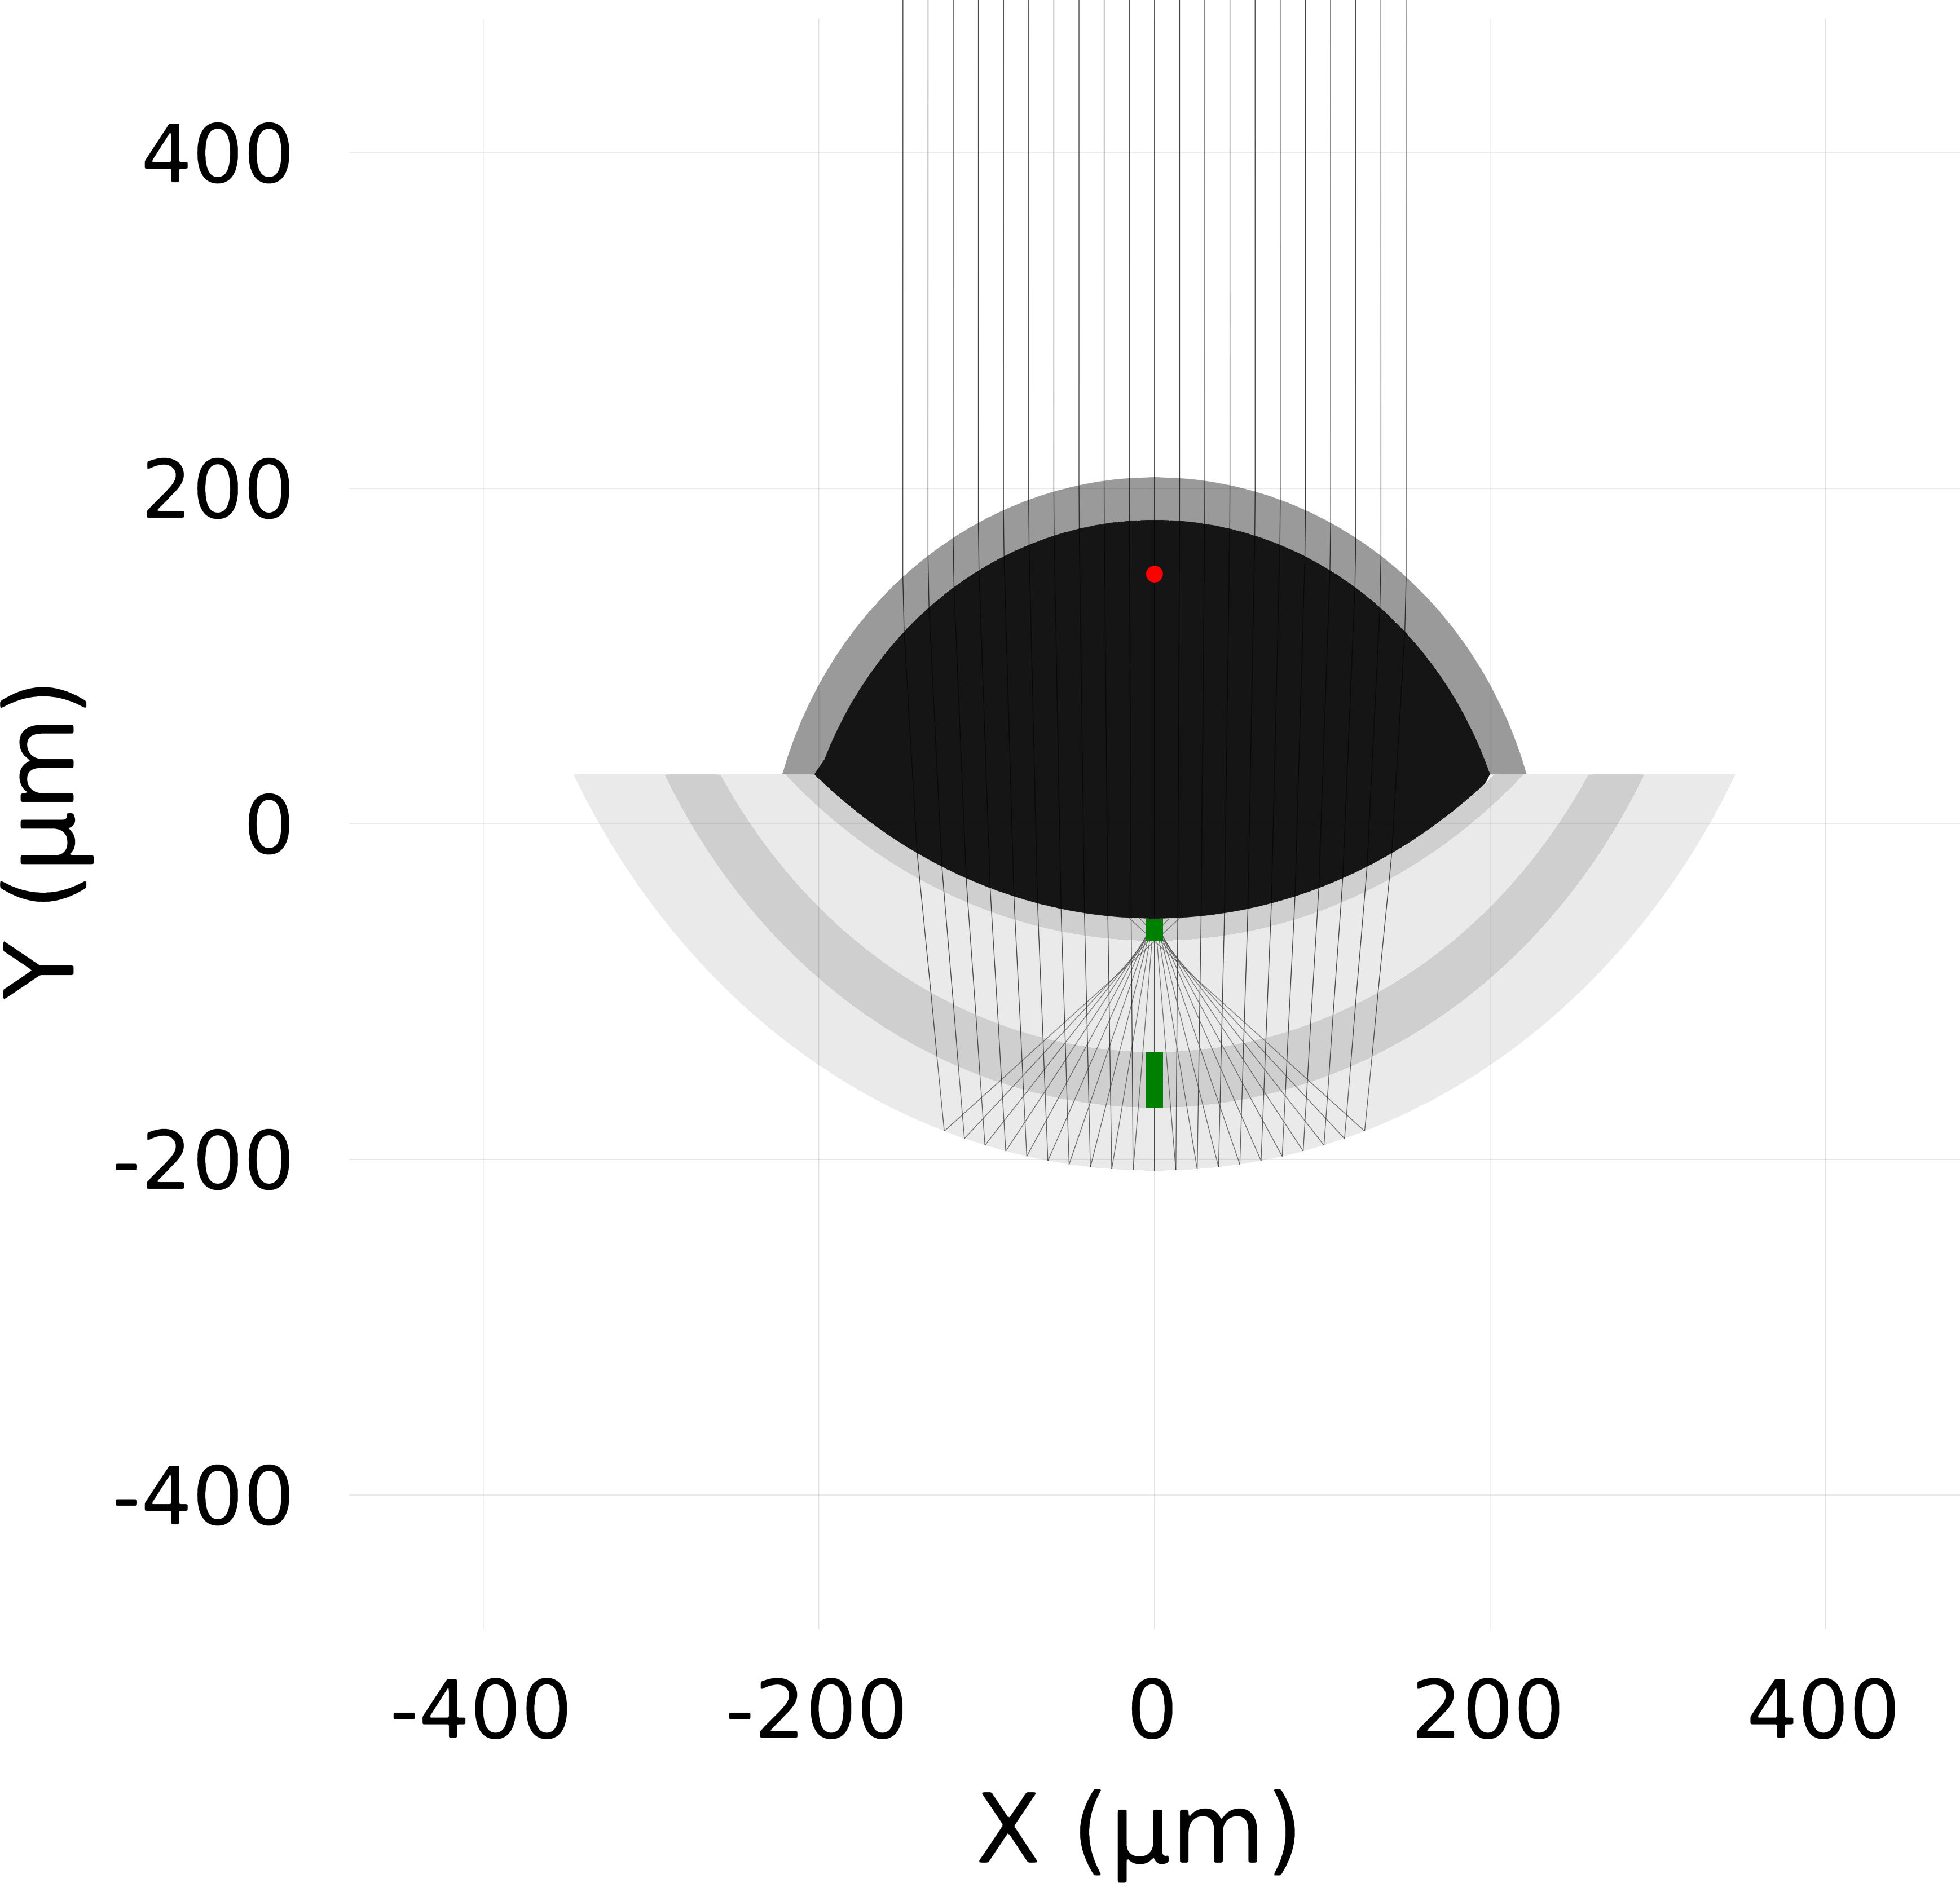
\includegraphics[width=0.95\textwidth]{img/normal}
    \end{center}

    \begin{center}
        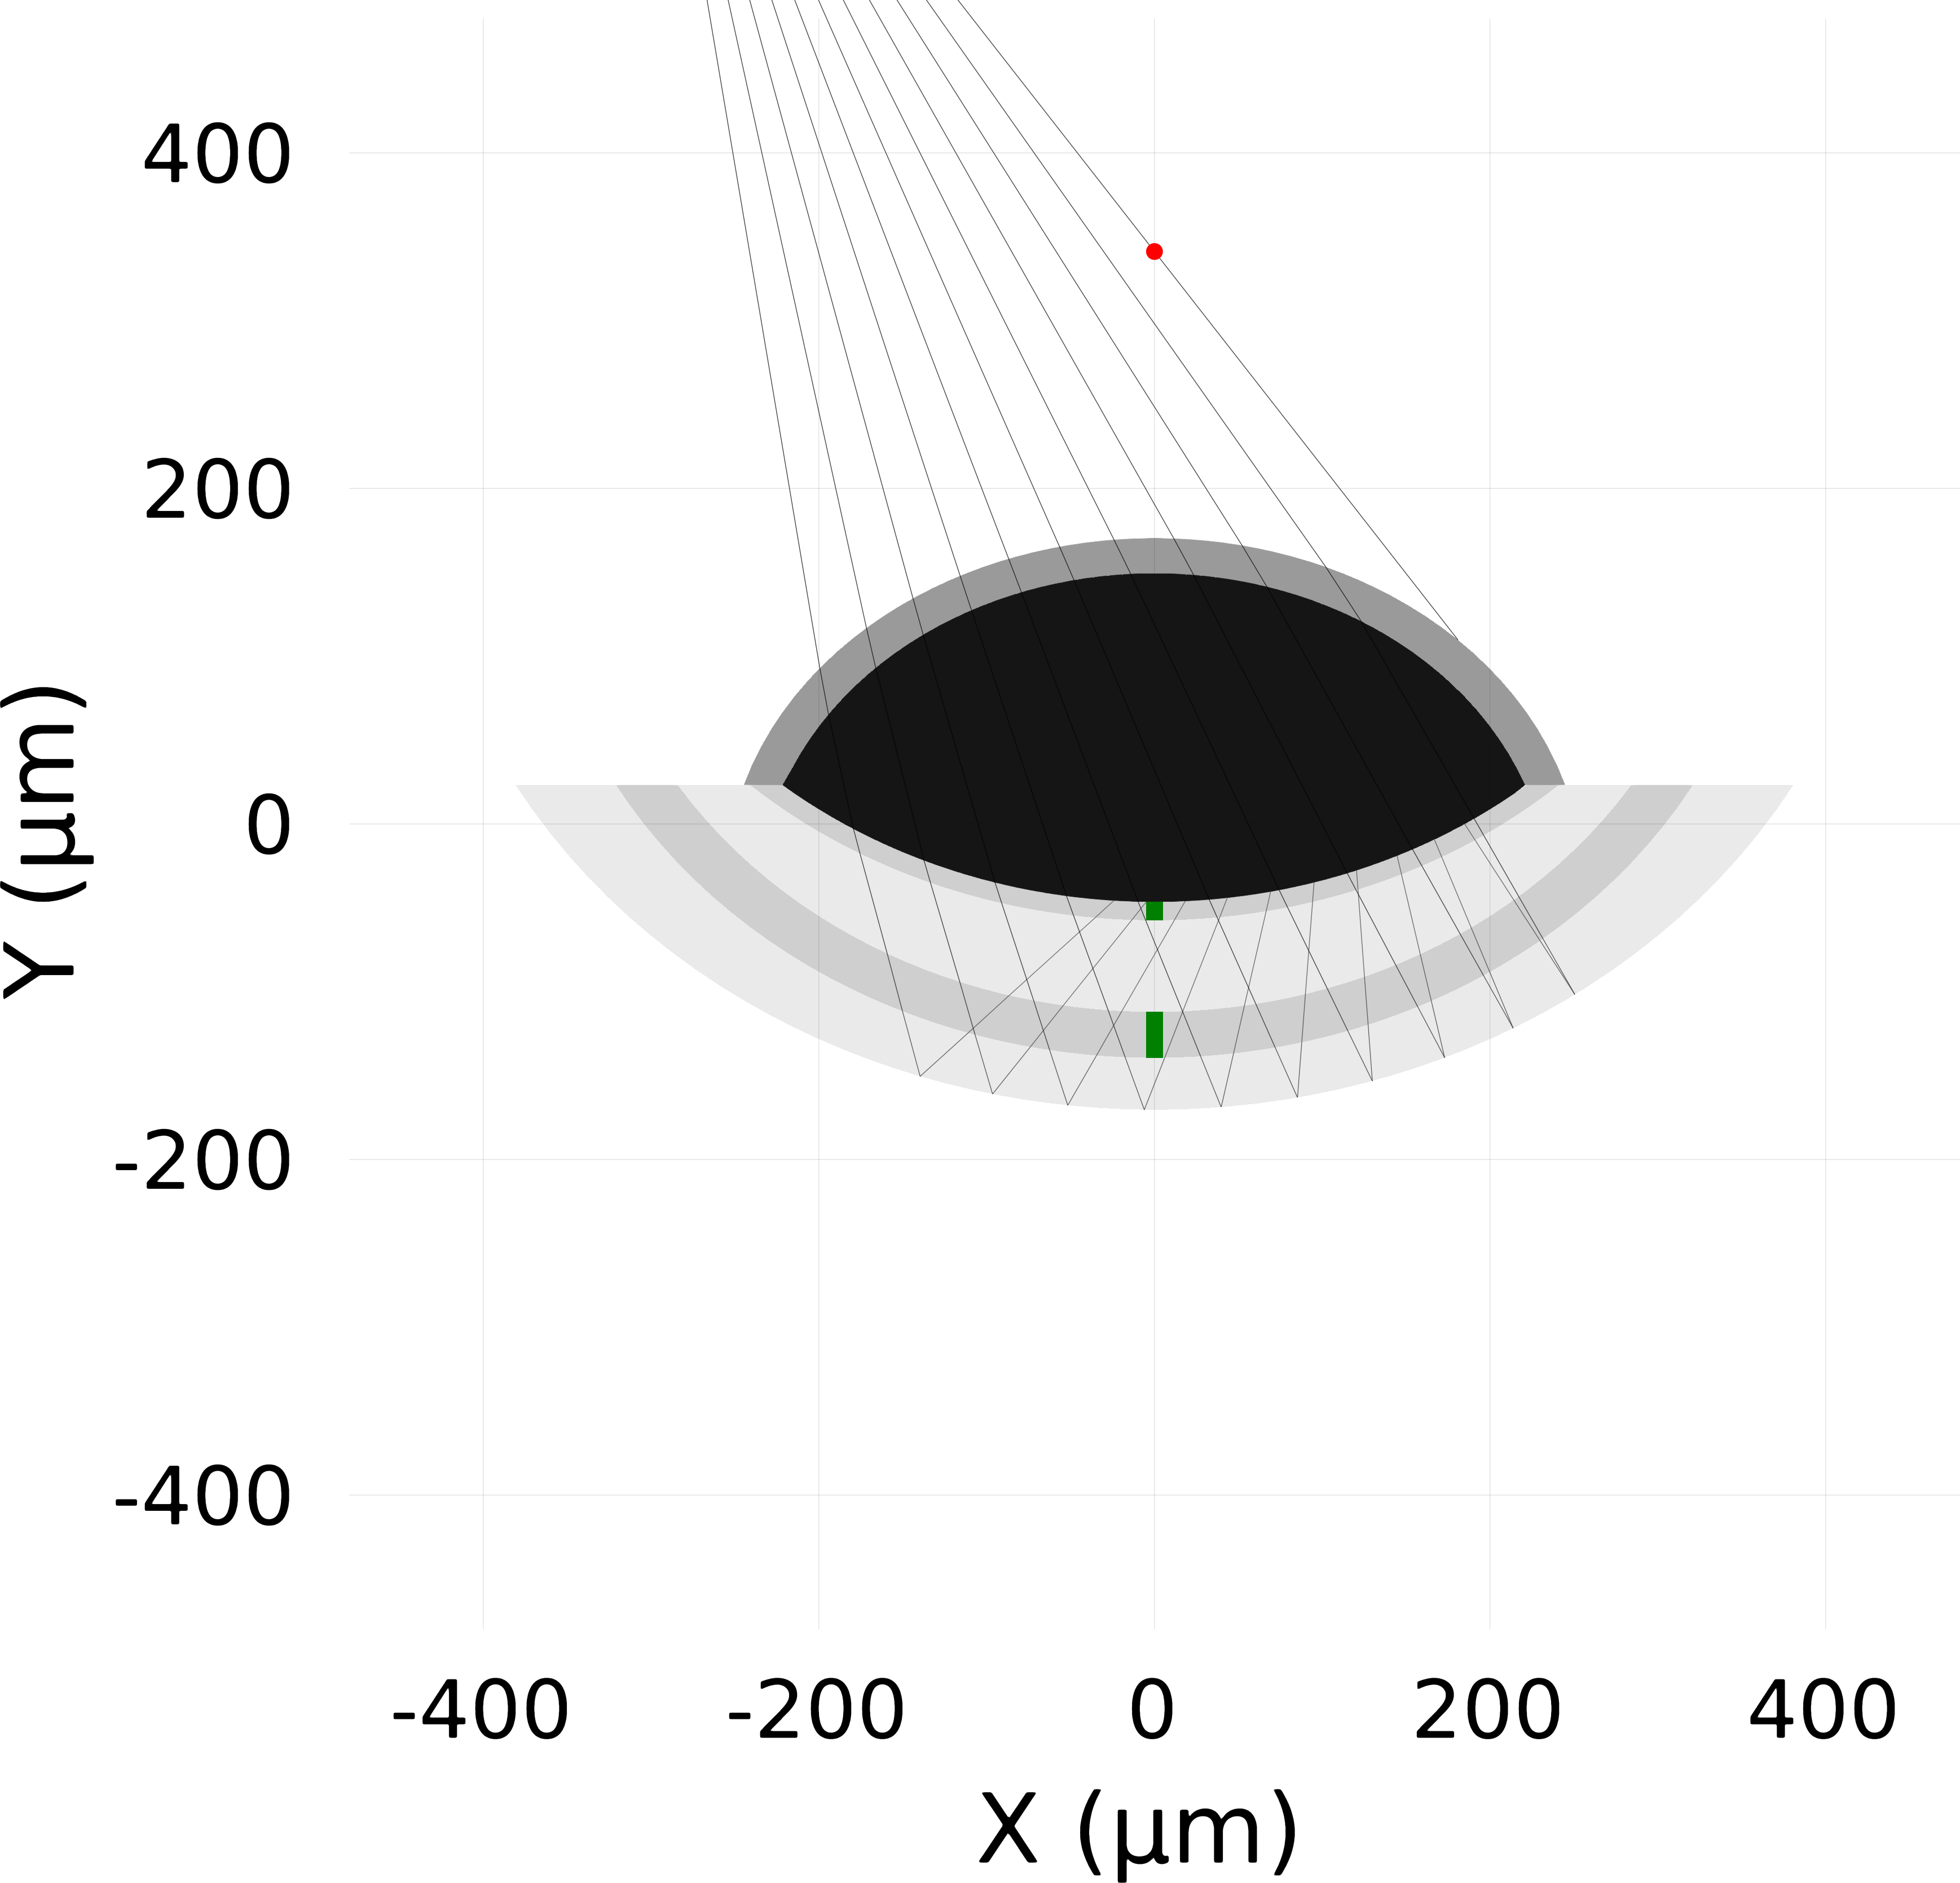
\includegraphics[width=0.95\textwidth]{img/abnormal}
    \end{center}

}
\end{document}
